%\documentclass[Serif, 10pt, brown, handout]{beamer} % Disable overlays for handout format
%\documentclass[Serif, 10pt, brown, handout, notes]{beamer} % Disable overlays for handout format and print notes
\documentclass[Serif, 10pt, brown]{beamer}
\usepackage{booktabs,xcolor}
%\usepackage[svgnames,table]{xcolor}
%\usepackage[tableposition=above]{caption}
\usepackage{pifont}
\newcommand*\CHECK{\ding{51}}
\usepackage{array}
\newcolumntype{P}[1]{>{\centering\arraybackslash}p{#1}}
%
\usepackage{setspace,mathtools,amssymb,multirow,array,amsmath,tikz}
\usepackage[normalsize]{subfigure}
\usetikzlibrary{patterns}
\usetikzlibrary{automata,positioning,decorations.pathreplacing,decorations}

\usepackage{curves}
\usepackage{wasysym}
\usepackage{epsfig,epstopdf,graphicx}

\curvewarnfalse
%
\newtheorem{proposition}{Proposition}
\theoremstyle{example}
\newtheorem{theoremh}{Theorem}
\theoremstyle{plain}
\renewcommand{\textfraction}{0.01}
\renewcommand{\floatpagefraction}{0.99}
\newcommand{\ul}{\underline}
\newcounter{units}
%
\usepackage[round]{natbib}
 \bibpunct[, ]{(}{)}{,}{a}{}{,}%
 \def\bibfont{\small}%
 \def\bibsep{\smallskipamount}%
 \def\bibhang{24pt}%
 \def\newblock{\ }%
 \def\BIBand{and}%
%
\setbeamercovered{dynamic}
% Logo
\logo{
\includegraphics[width=0.5in,keepaspectratio]{iitb_logo.png}}
%
% Setup
\mode<presentation>
	{
\usetheme[right,currentsection, hideothersubsections]{UTD}
			\useoutertheme{sidebar} \useinnertheme[shadow]{rounded}
			\usecolortheme{whale} \usecolortheme{orchid}
			\usefonttheme[onlymath]{serif}
			\setbeamertemplate{footline}{\centerline{Slide \insertframenumber/\inserttotalframenumber}}
	}
%
% Title
\usebeamercolor[fg]{author in sidebar}
\title[{Image Compression}]{\sc Image Compression Project}
\author[\ul{Authors}]{{\bf Saksham Rathi, Kavya Gupta, Shravan Srinivasa Raghavan}\\ \hspace{-1cm} (22B1003) \hspace{0.7cm} (22B1053) \hspace{1.7cm} (22B1054)}
\institute[UTD]{\sc\small CS663: Digital Image Processing\\ Under Prof. Ajit Rajwade}
\date[UCI]{Indian Institute of Technology Bombay \\ Autumn 2024}
%
%Presentation
\begin{document}
\frame{\titlepage}
%
%
%Slides

%TOC

\begin{frame}
	\transblindsvertical
	\frametitle{Contents}
	\tableofcontents[hidesubsections]
\end{frame}
\note[itemize]{
\item Here's the overall structure of my talk today.
}


% Introduction
\section[Problem Statement]{Problem Statement}
% 
% \setbeamercolor{background canvas}{use=structure,bg=white}
% \setbeamercolor{background}{use=structure,bg=white}
\begin{frame}{Problem Statement}
	The problem statement of this project has been taken from the following website:
	\begin{center}
		\href{https://www.cse.iitb.ac.in/~ajitvr/CS663_Fall2024/project.html}{\textcolor{blue}{\underline{CS663: Digital Image Processing}}}
	\end{center}

	We have built an image compression engine along the lines of the JPEG algorithm. Along with this, we have implemented PCA algorithm. We have also thoroughly studied a tier-1 conference paper {\bf Approximation and Compression With Sparse Orthonormal Transforms} and implemented the algorithm proposed in the paper.
	\vspace{1cm}

	All the algorithms were tested on a variety of image datasets. The results were compared and analyzed to understand the performance of the algorithms.
\end{frame}

\section{Basic Implementation}
\begin{frame}
	\frametitle{Basic Implementation}
	Here are the steps which were performed as part of the basic implementation:
	\begin{itemize}
		\item Computation of the 2D DCT coefficients of non-overlapping image patches
		\item Implementation of the quantization step
		\item Implementation of the Huffman tree
		\item Writing data to an appropriate file format (.bin) and plotting RMSE vs BPP
	\end{itemize}
	Here is the expression of RMSE:
	\begin{equation}
		\text{RMSE} = \sqrt{\frac{1}{N} \sum_{i=1}^{N}\sum_{j=1}^{M} (I_{\text{orig}}(i)(j) - I_{\text{recon}}(i)(j))^2}
	\end{equation}
	where $I_{\text{orig}}$ is the original image and $I_{\text{recon}}$ is the reconstructed image. BPP stands for the size of the image in bits divided by the number of pixels.
\end{frame}
\begin{frame}
	\frametitle{Quality Comparison}
	Here is the comparison of the reconstucted and the original image for a quality factor of 2:
	\begin{figure}
		\centering
		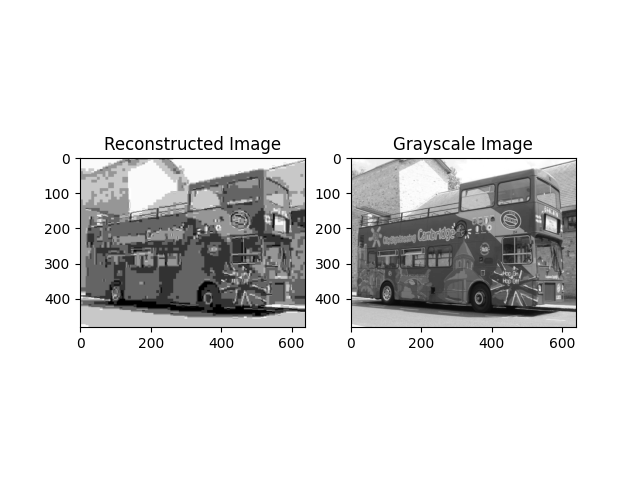
\includegraphics[width=0.7\textwidth]{../results/Quality: 2_comparison.png}
		\caption{Original and Reconstructed Image}
	\end{figure}
\end{frame}

\begin{frame}
	\frametitle{Quality Comparison}
	Here is the comparison of the reconstucted and the original image for a quality factor of 10:
	\begin{figure}
		\centering
		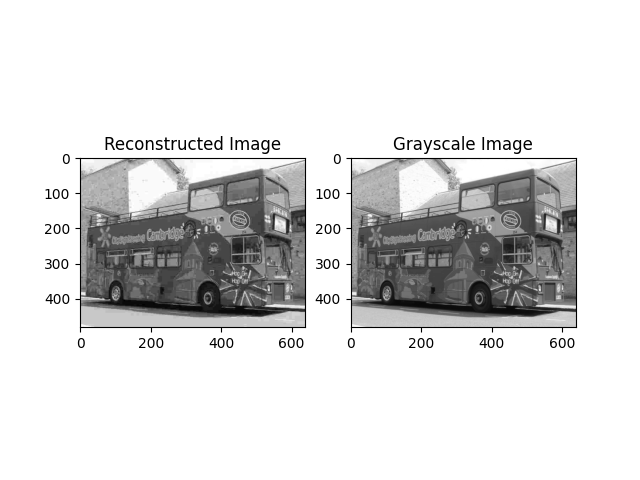
\includegraphics[width=0.7\textwidth]{../results/Quality: 10_comparison.png}
		\caption{Original and Reconstructed Image}
	\end{figure}
\end{frame}

\begin{frame}
	\frametitle{Quality Comparison}
	Here is the comparison of the reconstucted and the original image for a quality factor of 50:
	\begin{figure}
		\centering
		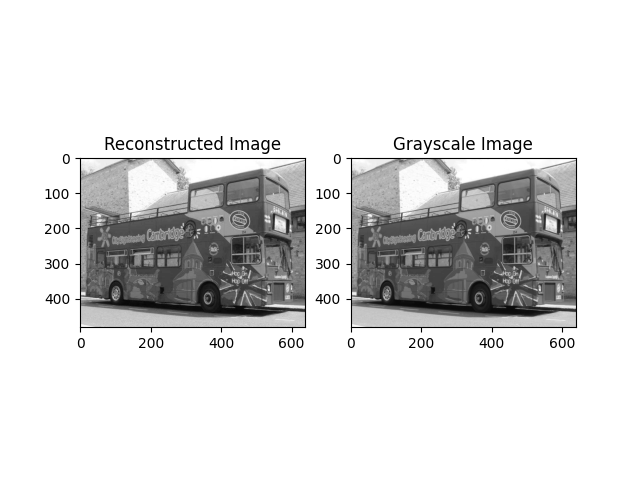
\includegraphics[width=0.7\textwidth]{../results/Quality: 50_comparison.png}
		\caption{Original and Reconstructed Image}
	\end{figure}
\end{frame}

\begin{frame}
	\frametitle{Quality Comparison}
	Here is the comparison of the reconstucted and the original image for a quality factor of 80:
	\begin{figure}
		\centering
		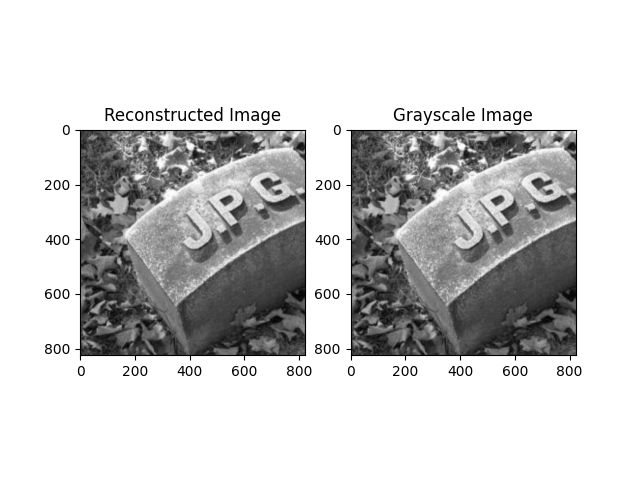
\includegraphics[width=0.7\textwidth]{../results/Quality: 80_comparison.png}
		\caption{Original and Reconstructed Image}
	\end{figure}
\end{frame}

\begin{frame}
	\frametitle{RMSE vs BPP}
	For the basic implementation, we have used the dataset from the miscellaneous category of the msrcorid dataset. We picked random 20 images and used 20 quality factors (in the range of 1 to 100) to plot the RMSE vs BPP graph. Here is the graph:

	\begin{figure}
		\centering
		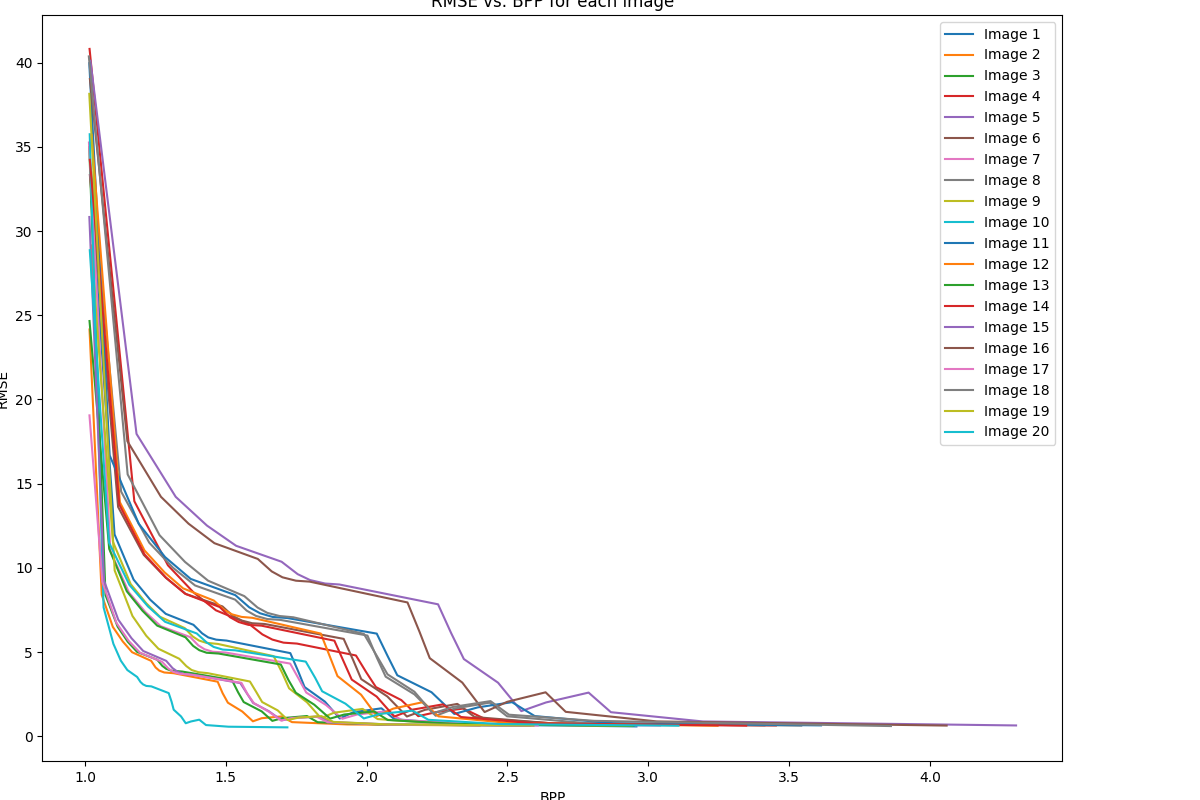
\includegraphics[width=0.7\textwidth]{../results/basic.png}
		\caption{RMSE vs BPP}
	\end{figure}
	
\end{frame}

\begin{frame}
	\frametitle{Comparison of Basic vs JPEG}
	The following plot shows how the basic algorithm performs as compared to the JPEG algorithm. 
	
	\begin{figure}
		\centering
		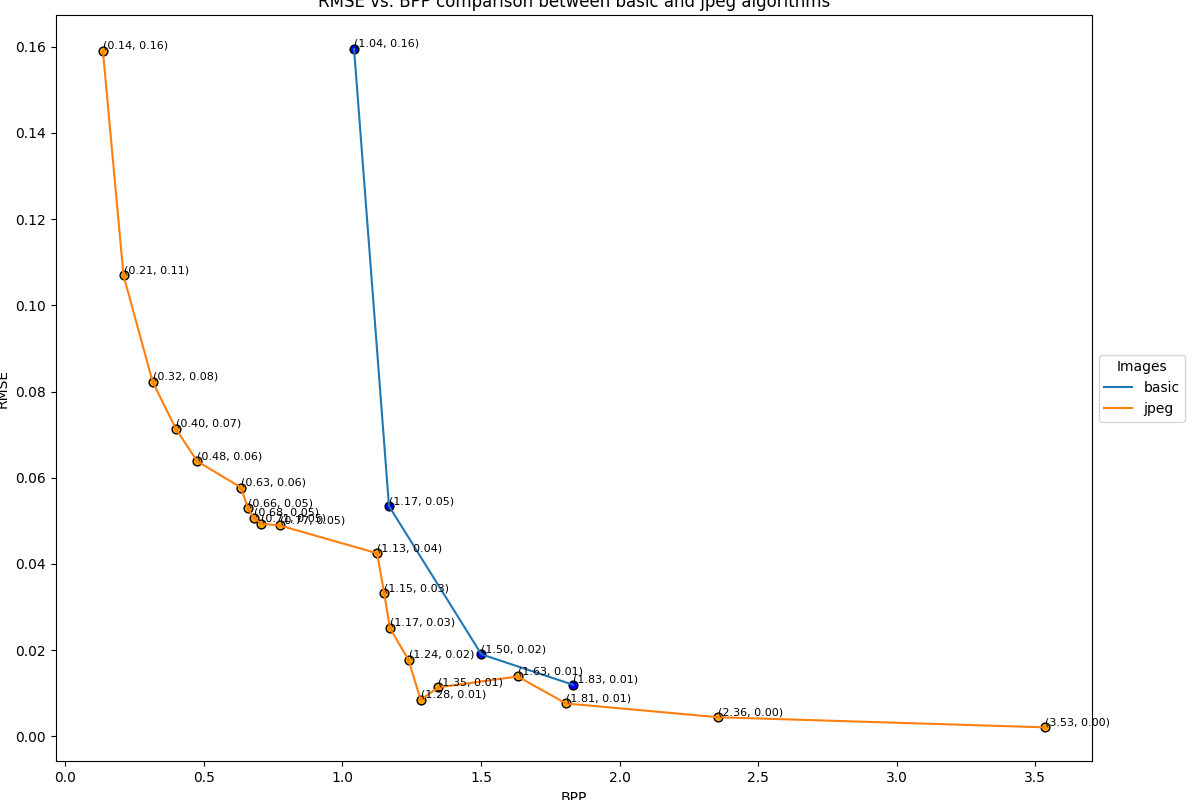
\includegraphics[width=0.7\textwidth]{../results/basic_jpeg_comparison.png}
		\caption{Comparison of Basic and JPEG}
	\end{figure}
\end{frame}

\section{Run Length Encoding}

\begin{frame}
	\frametitle{Run Length Encoding}
	The quantized DCT coefficients are arranged in a zigzag order. This pattern leaves a bunch of consecutive zeros at the end.

	\vspace{1cm}

	In runlength encoding, we replace the consecutive zeros with a pair of numbers: the number of zeros and the value of the next non-zero element. This reduces the size of the data to be stored.
\end{frame}

\begin{frame}{RMSE vs BPP}
	The dataset of images from the miscellaneous category of the msrcorid dataset was used to plot the RMSE vs BPP graph. Here is the graph:

	\begin{figure}
		\centering
		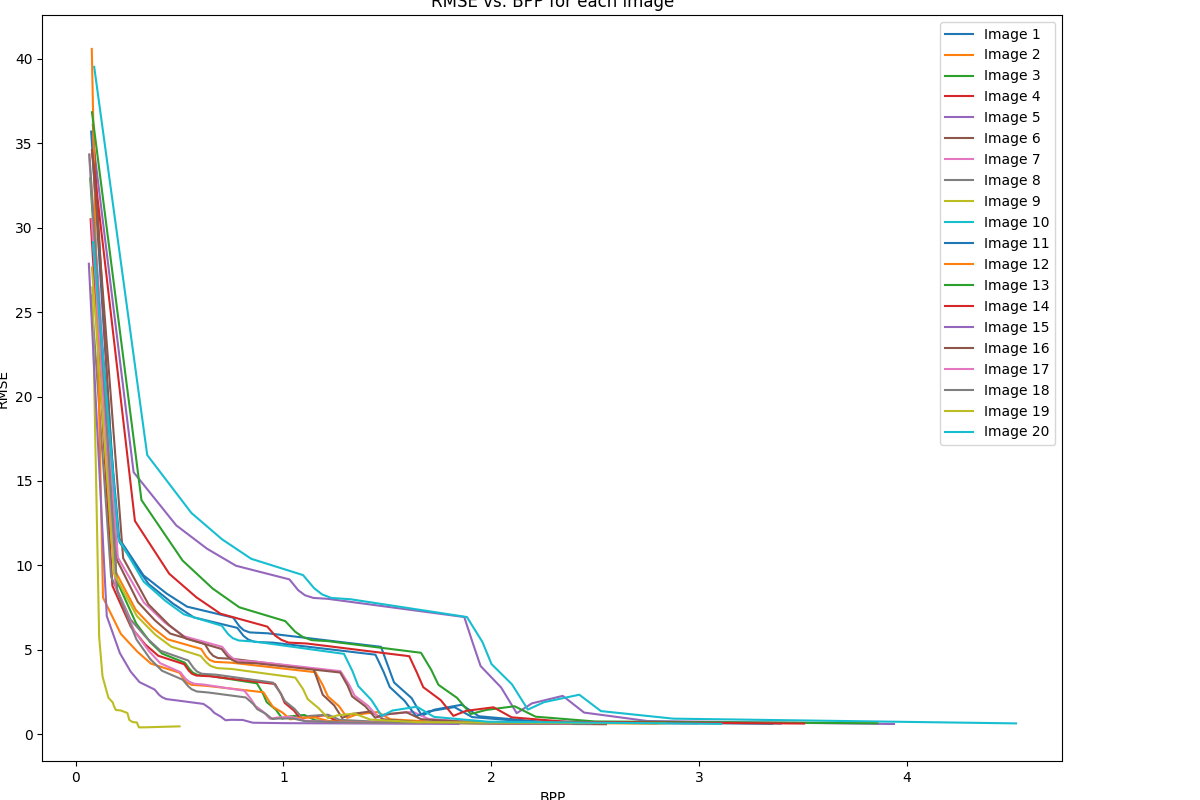
\includegraphics[width=0.7\textwidth]{../results/runlength.png}
		\caption{RMSE vs BPP}
	\end{figure}

\end{frame}

% \section{Comparison of Basic and Run Length Encoding}
\begin{frame}
	\frametitle{Comparison of Basic and Run Length Encoding}

	\begin{figure}
		\centering
		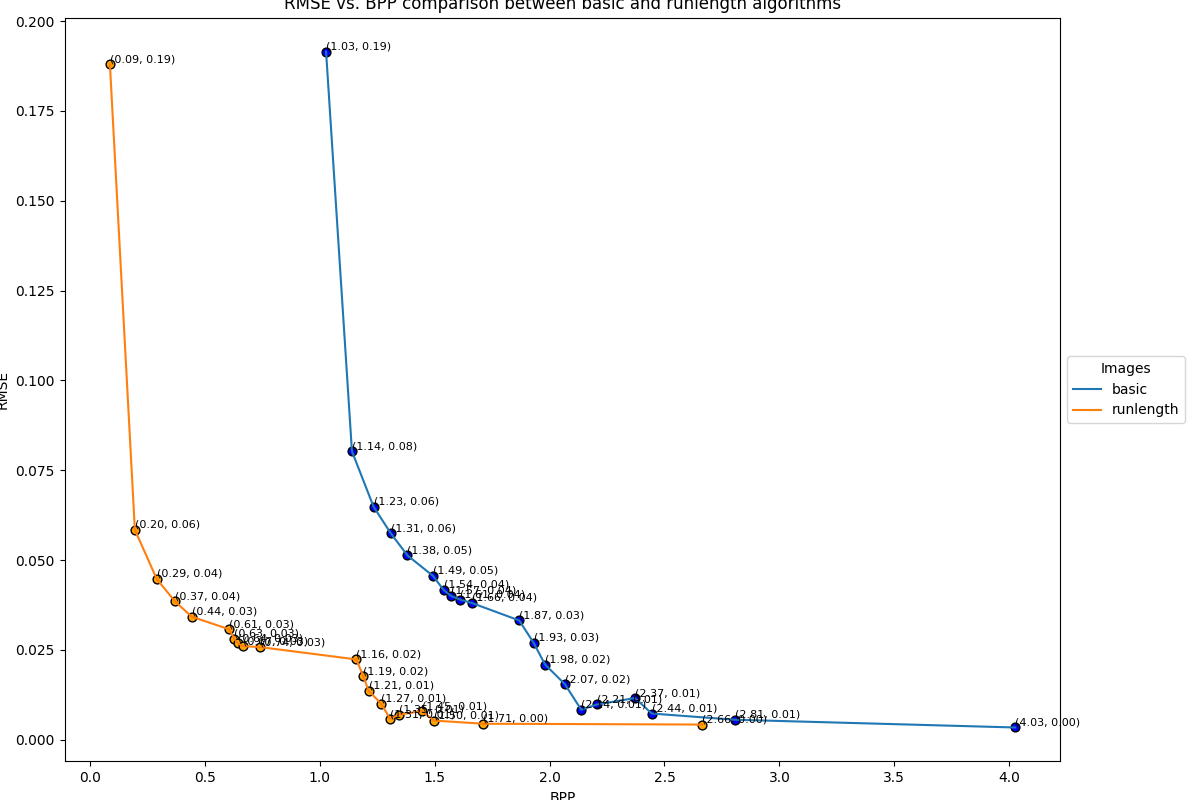
\includegraphics[width=0.7\textwidth]{../results/basic_runlength_comparison.png}
		\caption{Comparison of Basic and Run Length Encoding}
	\end{figure}
\end{frame}

\begin{frame}
	\frametitle{Comparison of Run Length Encoding and JPEG Algorithm}

	\begin{figure}
		\centering
		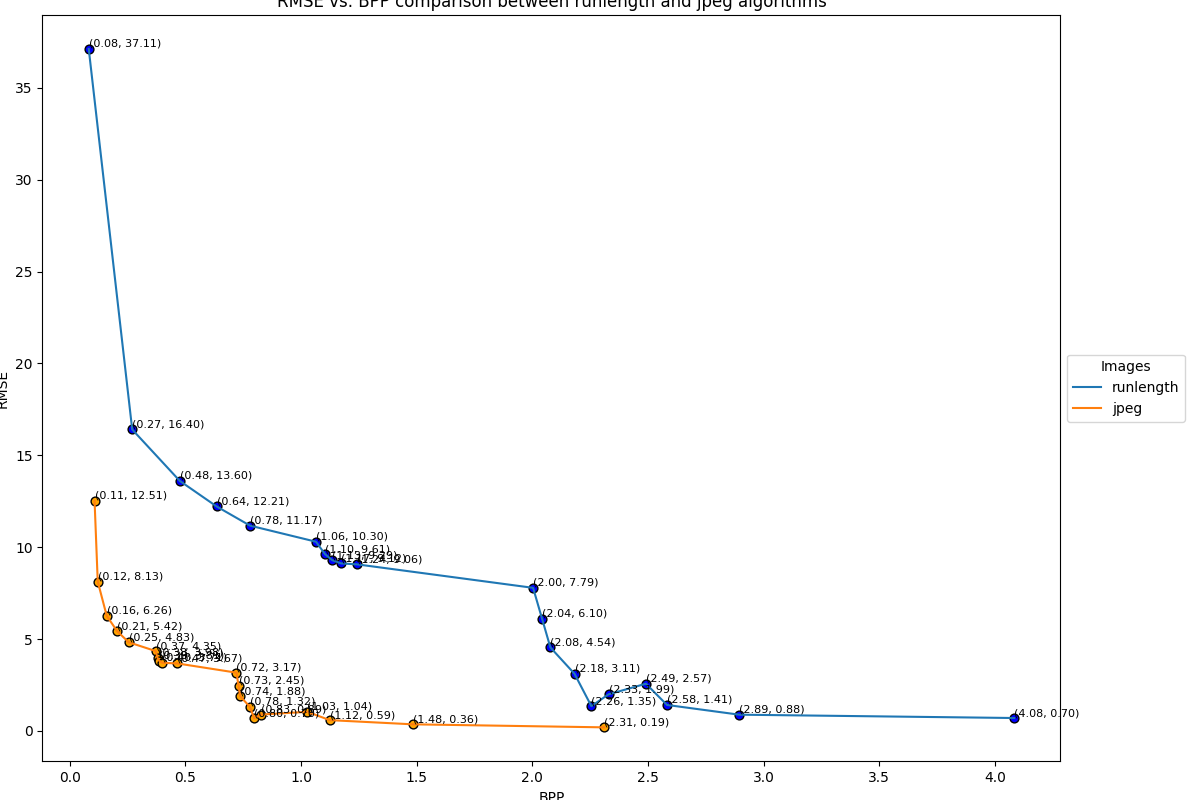
\includegraphics[width=0.7\textwidth]{../results/runlength_jpeg_comparison.png}
		\caption{Comparison of Basic and Run Length Encoding}
	\end{figure}
\end{frame}




\section{Individual Contributions}

\begin{frame}
	\frametitle{Individual Contributions}
	\begin{alertblock}{Saksham Rathi}
	\end{alertblock}
	\begin{alertblock}{Kavya Gupta}
	\end{alertblock}
	\begin{alertblock}{Shravan Srinivasa Raghavan}
	\end{alertblock}

\end{frame}
\section{Conclusion}
\begin{frame}
	\frametitle{Conclusion}
\end{frame}

\section{References}

\begin{frame}
	\frametitle{References}
	\begin{itemize}
		\item \href{https://docs.google.com/presentation/d/1-8xCg7o8Vtc9ghJf6y1Nkq9-TV0qSNfX/edit?usp=sharing&ouid=115909013767952805958&rtpof=true&sd=true}{\textcolor{blue}{\underline{CS663: Image Compression Slides}}}
		\item Course Textbook: ``Digital Image Processing'' by Rafael C. Gonzalez and Richard Woods, 3rd edition
		\item Osman Gokhan Sezer, Onur G. Guleryuz and Yucel Altunbasak, ``Approximation and Compression With Sparse Orthonormal Transforms'', IEEE Transactions on Image Processing, 2015
		\item \href{https://github.com/jeremyfell/image-compression/blob/master/image-compression.py}{\textcolor{blue}{\underline{Sample Image Compression Code}}}
		\item \href{https://github.com/adl1995/edge-detectors/blob/master/marr-hildreth-edge.py}{\textcolor{blue}{\underline{Marr-Hildreth Edge Detector}}}
	\end{itemize}
\end{frame}

\end{document}


